\documentclass[11pt]{article}

\usepackage{pdfpages}
\usepackage{hyperref}
\usepackage{enumerate}
\usepackage{listings}
\usepackage{float}

\renewcommand*\ttdefault{lmtt}
\renewcommand*\sfdefault{lmss}
\renewcommand{\familydefault}{\sfdefault}

\begin{document}

\author{\textbf{Group 8} \\* Arian Barakat \\* Hao Chi KIANG}

\title{Laboratory Work 1}
\maketitle

\section*{Assignment 1}

\begin{figure}[H]
  \centering
   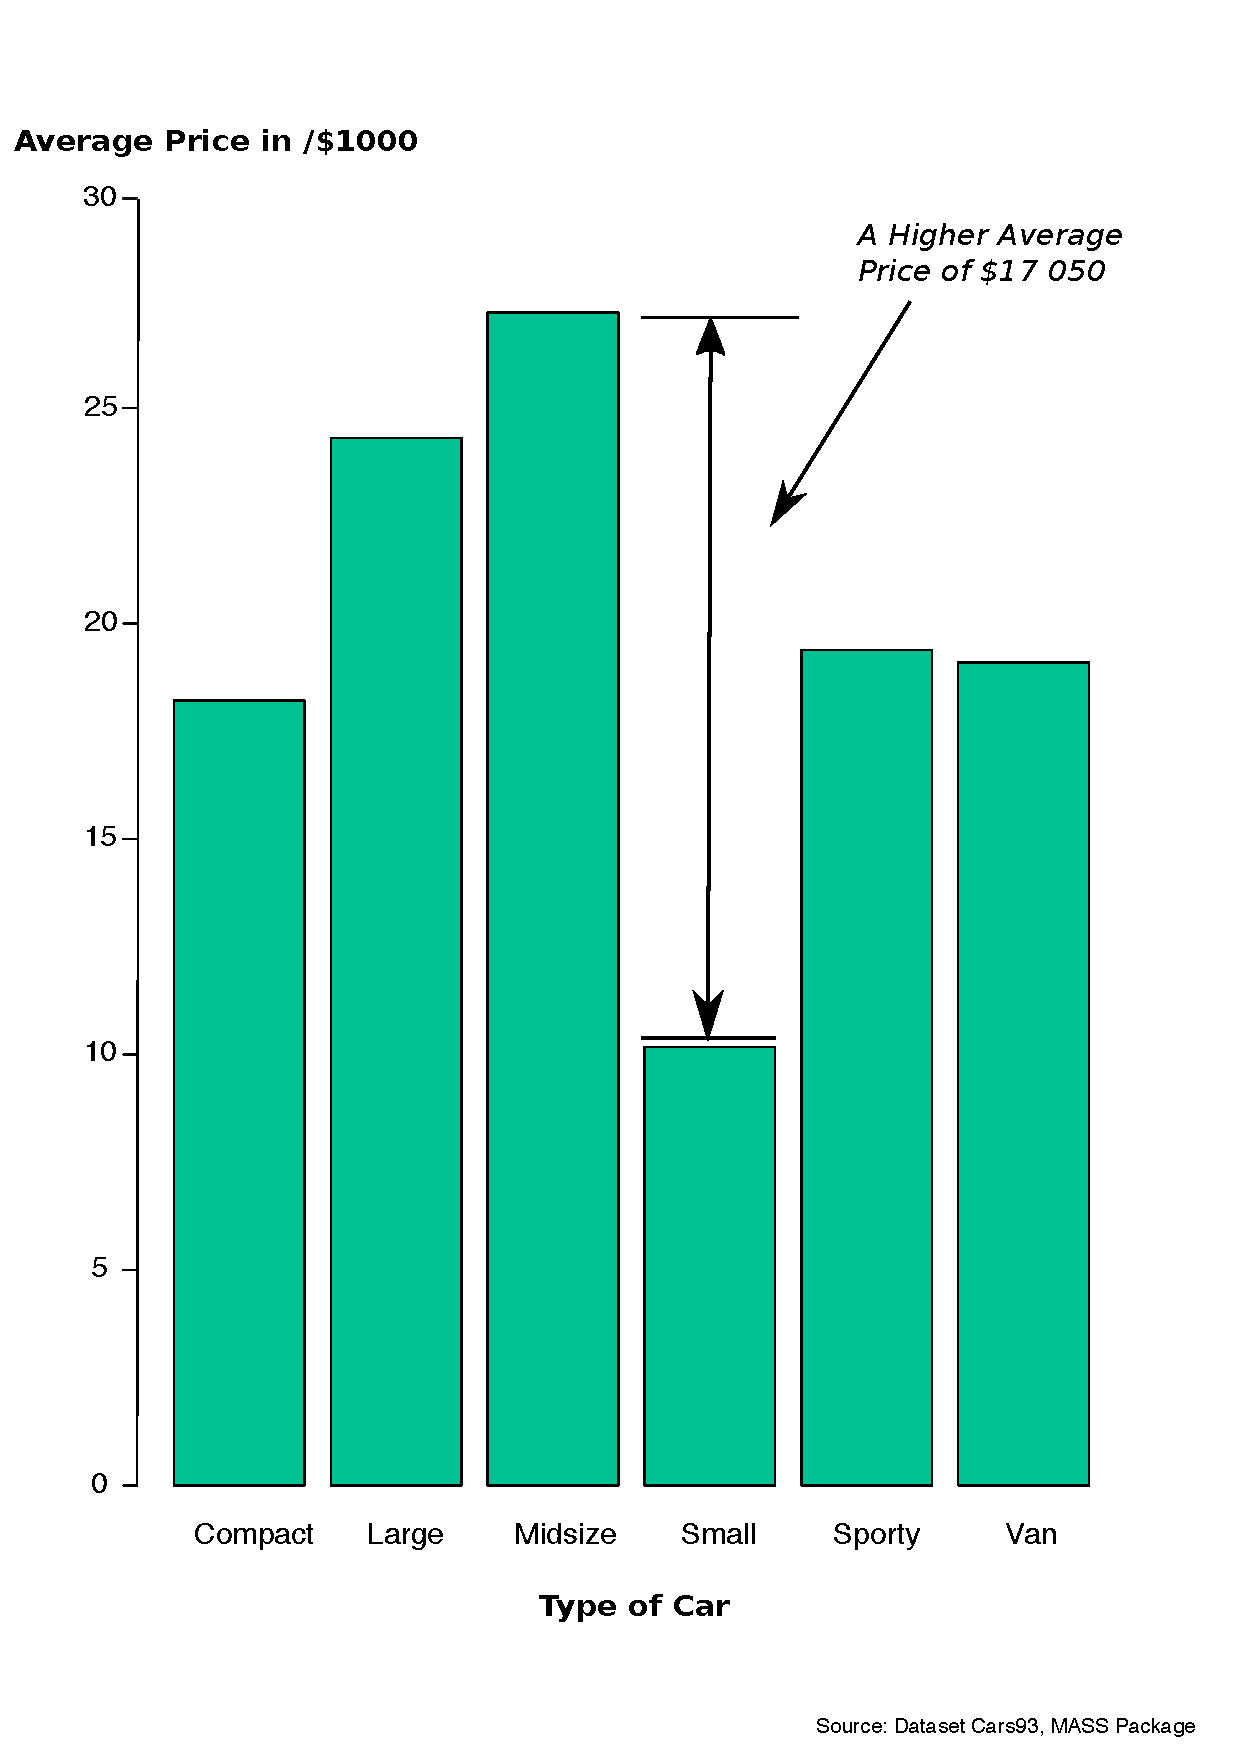
\includegraphics[scale=0.4]{Assignment_1.pdf}
   \caption{The Average Car Price for each type of Car}
\end{figure}


\section*{Assignment 2}

% TODO: Adjust the picture so that it centres in the page

\begin{figure}[H]
  \centering
  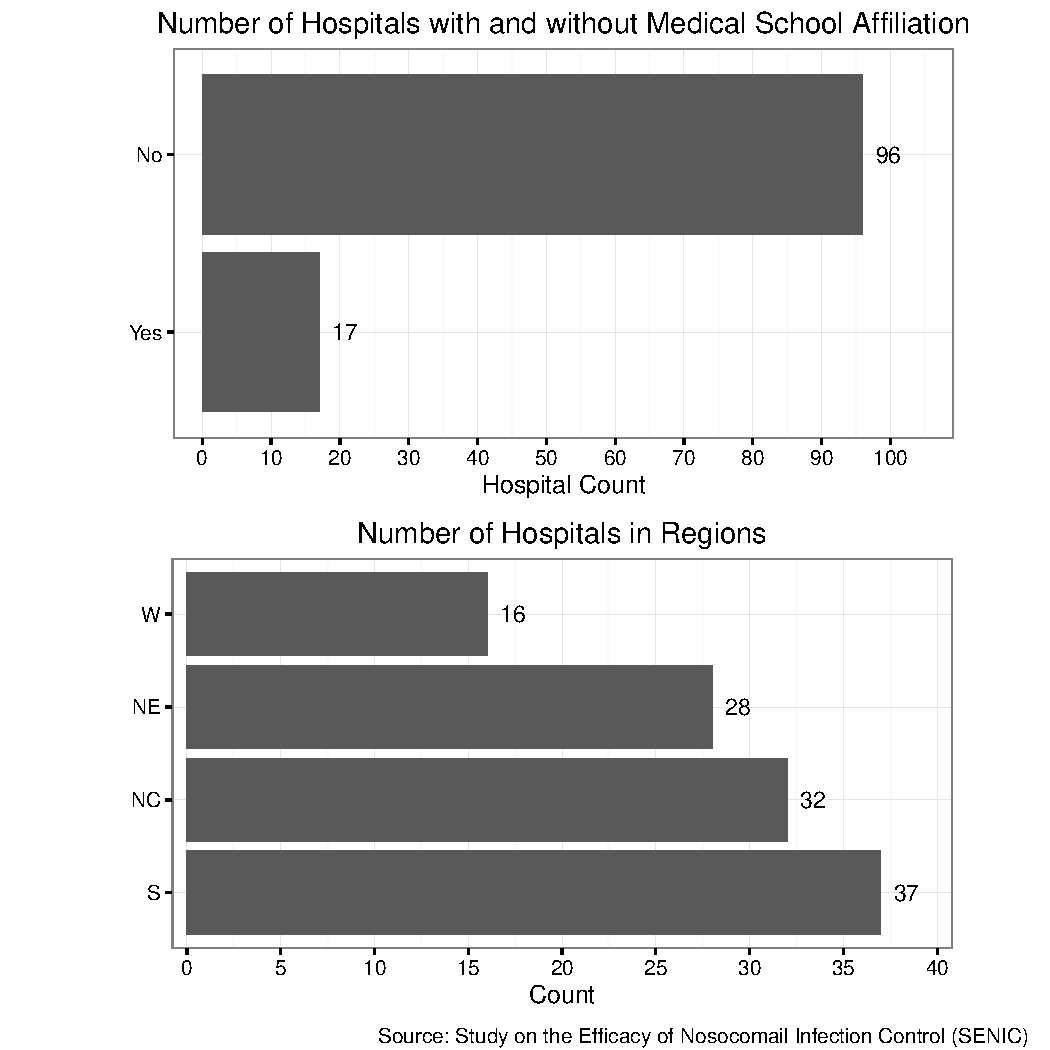
\includegraphics[scale=0.8]{qualitative_vars.pdf}
  \caption{Count of observations of the two
    qualitative variables}
  \label{fig:qualivars}
\end{figure}

There are only two qualitative variables among all: the Medical School
Affiliation (X7) and Region (X8). \autoref{fig:qualivars} is the combined
chart requested.

We can observe from \autoref{fig:qualivars} that:
\begin{enumerate}
\item
  Only a few hospitals have affiliation with medical schools.
\item
  The number of hospital in a region varies a lot across regions. This
  does not tell us anything meaningful, however, unless this count is
  normalized by the population size of each regions. So if this is an
  real analysis, the next step may be to construct a graph of the ratio
  'hospital number/population-size', or even better
  'number of bed/population-size'.
\end{enumerate}



\begin{figure}[H]
  \centering
  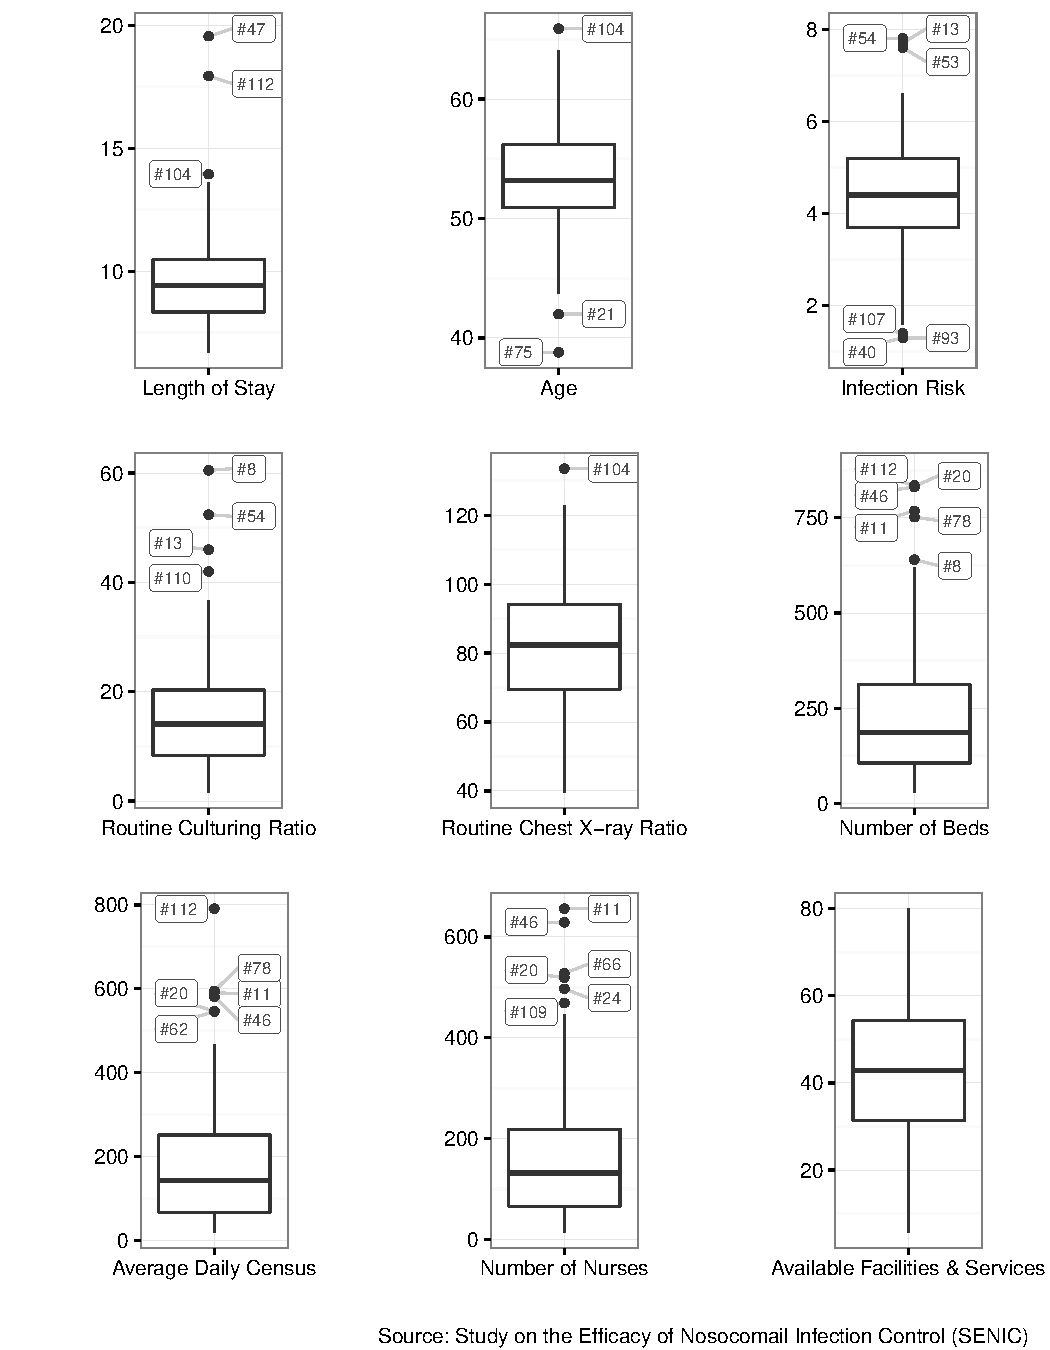
\includegraphics[scale=0.8]{quantitative_vars.pdf}
  \caption{Combined plot of all quantitative variables}\label{fig:quantvars}
\end{figure}

The quantitative variables are plotted in box plots in \autoref{fig:quantvars}.

The following are some observations:
\begin{enumerate}
\item
  Average length of stay varies among the hospitals from less than five days to
  near 20 days. This suggest that some hospitals does not have bed or service of
  taking many long-staying patients.
\item
  Both number of nurses, average daily census and number of beds ranges from
  several dozens to several hundreds. They also shares many outliers. This suggest
  some hospitals are having many staying patients and some hospitals doesn't take
  in many staying patients at all.
\item
  Hospital \#104 outlies in both length of stay and average age of patient. It
  seems that this hospital probably has a geriatric or paliative care service.
  Its outlying in routine chest X-ray ratio may be related to this as well.
\item
  Hospital \#13 and \#54 outlies together in both infection risk and routine culturing
  ratio. Both intuition and this coincidence leads us to suspect there is correlation
  between culturing and infection. Ploting them in a scatter plot may help us find
  this out.
\end{enumerate}


\section*{Assignment 3}

\label{subsec:nurse2bed}
\lstset{
  frame=single,
  basicstyle=\ttfamily\footnotesize,
  commentstyle=\color{gray},
  frame=L,
  language=R,
  showstringspaces=false,
}

\begin{lstlisting}[caption={Hospital with the lowest nurse-to-bed ratio}\label{lst:leastnurse}]
least_nurse_hospital <-
    senic_data[which.min(senic_data$X10/senic_data$X6),]

# Result:
#     Obs   X1   X2  X3  X4   X5  X6 X7 X8 X9 X10  X11
# 107 107 7.14 51.7 1.4 4.1 45.7 115 No  S 90  19 22.9
\end{lstlisting}


\autoref{lst:leastnurse} gives the hospital with the lowest nurse-to-bed ratio.
Hospital \#107 has 115 beds but only 19 nurses. The ratio is 0.165. This ratio
shows on average how many nurses a bed has. Staying patient should be better off
when this ratio is higher. Nurses seem to be short-staffed in this hospital.


\begin{figure}[H]
  \centering
   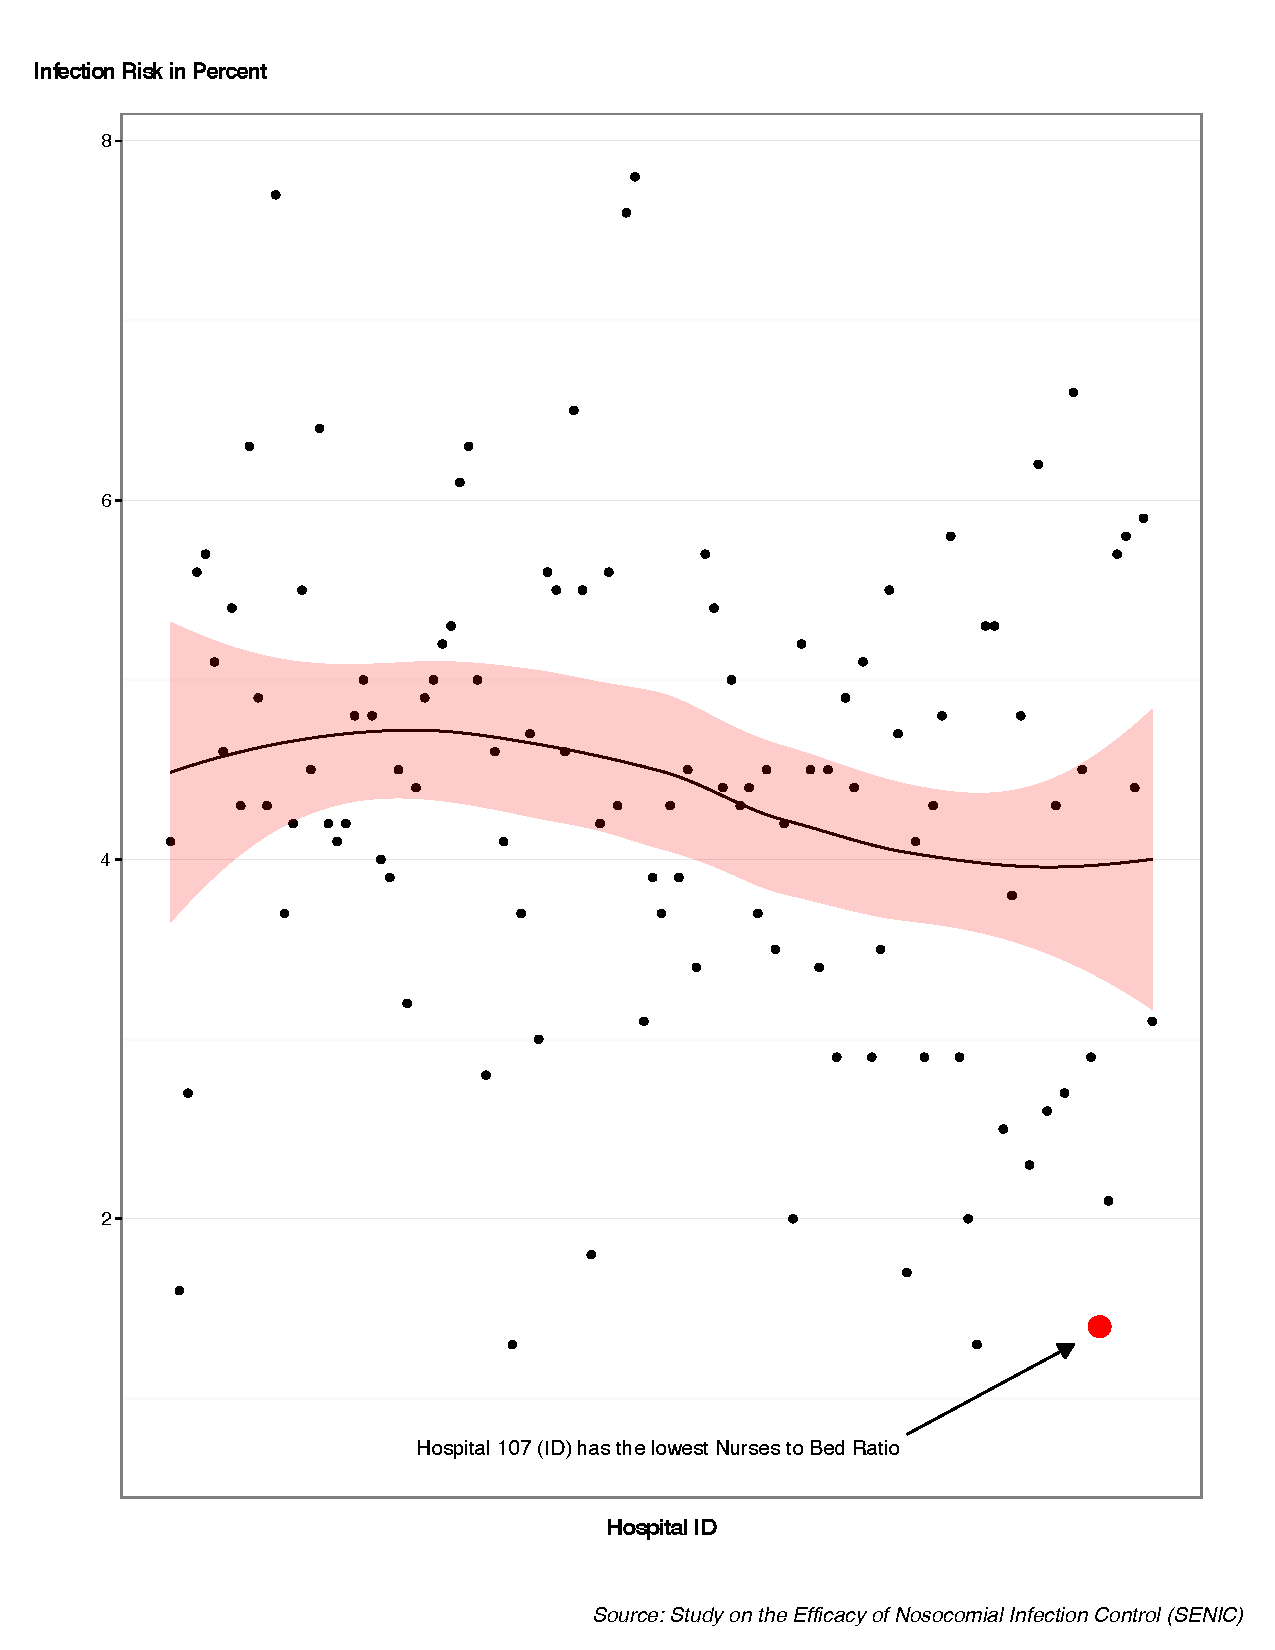
\includegraphics[scale=0.5]{Assignment_3.pdf}
   \caption{Infection Risk vs. Hospital ID, with LOESS Fitted Values and corresponding Confidence Interval. The hospital with the lowest \textit{Nurse-to-Bed Ratio} is marked out.}
   \label{fig:assignment3}
\end{figure}

From the \autoref{fig:assignment3}, the following remarks/conclusions can be made:

\begin{enumerate}
\item
Hospital \#107 has the lowest Nurse-to-Bed ratio, as previously mentioned, as well as one of the lowest Infection Risk of all of the studied hospitals. The low Nurse-to-Bed ratio may have an effect on the Infection Risk, but this cannot be concluded without further analysis. 
\item
By studying the figure above, a straight line appears to fit within the confidence interval for the \textit{LOESS curve}. A straight line would imply on a non-dependent relation between the two variables (\textit{Infection Risk} and \textit{Observation number}).
\end{enumerate}


\newpage

\section*{Appendix}

\begin{lstlisting}
###################################
## Course   : Visualization
## Lab      : 1
## Group    : 8
##
##
####################################
rm(list = ls())

##### Assignment 1

install.packages("MASS")
library(MASS)

data(Cars93, package = "MASS")
mydata_1 <- Cars93


df1=aggregate(Price~Type, data=mydata_1, FUN=mean)
barplot(df1$Price, names.arg=df1$Type)



##### Assignment 2

library(ggplot2)
library(grid)
library(gridExtra)
library(FField)
library(scales)

## Some initial settings
senic_path <- 'data/Senic.csv'   # Path to the data file
SENIC.ref <-
    "Source: Study on the Efficacy of Nosocomail Infection Control (SENIC)"
theme_set( theme_bw() )                 # ggplot appearance


#### 2.2: Qualitative plots
senic_data <- read.csv2(senic_path)
senic_data$X7 <- factor(senic_data$X7,
                        levels=c(1,2),
                        labels=c('Yes', 'No'),
                        ordered = TRUE)
senic_data$X8 <- factor(senic_data$X8,
                        levels=c(1,2,3,4),
                        labels=c('NE', 'NC', 'S', 'W'))

senic_column_desc <-
    list(Obs = 'Identification Number',
         X1 = 'Length of Stay',
         X2 = 'Age',
         X3 = 'Infection Risk',
         X4 = 'Routine Culturing Ratio',
         X5 = 'Routine Chest X-ray Ratio',
         X6 = 'Number of Beds',
         X7 = 'Medical School Affiliation',
         X8 = 'Region',
         X9 = 'Average Daily Census',
         X10 = 'Number of Nurses',
         X11 = 'Available Facilities & Services')

## 2.2: Qualitative plots
plot_x7 <- ggplot(senic_data, aes(X7)) +
    geom_bar( stat = 'count' ) +
    geom_text( stat = 'count', aes(label=..count..), hjust = -0.5) +
    ggtitle(
        paste('Number of Hospitals with', # Line too long
              'and without Medical School Affiliation',
              sep = '') +
    xlab('') +
    ylab('Hospital Count') +
    coord_flip() +
    scale_y_continuous(
        expand = c(0.04, 0),
        limits = c(0, 105),
        breaks = scales::pretty_breaks(n=10) ) +
    theme( aspect.ratio = 1/2 )

plot_x8 <- ggplot(senic_data, aes(reorder(X8, -table(X8)[X8]))) +
    geom_bar( stat = 'count' ) +
    geom_text( stat = 'count', aes(label=..count..), hjust = -0.5) +
    ggtitle('Number of Hospitals in Regions') +
    xlab('') +
    ylab('Count') +
    coord_flip() +
    scale_y_continuous(
        expand = c(0.02, 0),
        limits = c(0, 40),
        breaks = scales::pretty_breaks(n=10) ) +
    theme( aspect.ratio = 1/2 )


plot_quali_vars <- grid.arrange(
    plot_x7,
    plot_x8,
    nrow = 2,
    bottom = textGrob(SENIC.ref,
                      gp = gpar(fontface=1, fontsize=10),
                      hjust=1,
                      x=0.98)
)


## Export
## ggsave('senic_x7.pdf', plot_x7)
## ggsave('senic_x8.pdf', plot_x8)
ggsave('../qualitative_vars.pdf', plot_quali_vars)




#### 2.3: Quantitative plots

boxplot_aspectratio <- 2.4

make_quant_boxplot <- function (colname) {
    # Outliers position
    outliers.leftpos <- 0.60
    outliers.rightpos <- 1.16

    ## Normalizatio factors before passing coordinates to orce
    ## field factor for FField library

    ## 70 because y axis should have stronger field
    y.fact <- 70 / max(senic_data[ ,colname])
    x.fact <- 100 / outliers.rightpos


    # Data frame for holding outliers labels data
    column <- senic_data[ ,colname]
    outliers.frame <-
        data.frame(
            outliers_mask =
                column < quantile(column, 0.25) - 1.5 * IQR(column)
                | quantile(column, 0.75) + 1.5 * IQR(column) < column
        )

    outliers.frame$outliers =
        ifelse(
            outliers.frame$outliers_mask,
            paste('#', senic_data$Obs, sep = ''),
            NA )

    n_outliers = nrow( outliers.frame[outliers.frame$outliers_mask, ] )

    outliers.frame$xcoord = rep(NA, nrow(outliers.frame))
    outliers.frame$xcoord.t = rep(NA, nrow(outliers.frame))
    outliers.frame$ycoord.t = rep(NA, nrow(outliers.frame))

    outliers.frame$xcoord[outliers.frame$outliers_mask] =
        c(
            matrix(c(rep(outliers.rightpos, floor(n_outliers / 2)),
                     rep(outliers.leftpos, floor(n_outliers / 2))),
                   2, byrow = T),
            rep(outliers.rightpos, n_outliers - floor(n_outliers / 2) * 2 )
        )

    outliers.frame[outliers.frame$outliers_mask, colname] <-
        senic_data[outliers.frame$outliers_mask, colname]

    outliers.frame$xcoord.t <- outliers.frame$xcoord * x.fact
    outliers.frame$ycoord.t[outliers.frame$outliers_mask] <-
        senic_data[outliers.frame$outliers_mask, colname] * y.fact

    outliers.frame <- cbind(
        outliers.frame,
        FFieldPtRep(
            coords = outliers.frame[ ,c("xcoord.t", "ycoord.t")],
            rep.fact = 43
        )
    )

    # Detect moved x-coordinate. Kind of a hacky way to posit the labels
    outliers.frame$x <- ifelse( outliers.frame$x < 1.01 * x.fact,
                                outliers.leftpos,
                                outliers.rightpos )
    outliers.frame$y <- outliers.frame$y / y.fact

    plot <- ggplot(senic_data,
                   aes_string(x = shQuote(senic_column_desc[[colname]]),
                              y=colname)) +
        geom_segment(
            data = outliers.frame,
            aes_string(x = "x",
                       xend = shQuote(senic_column_desc[[colname]]),
                       y = "y",
                       yend = colname),
            na.rm = TRUE,
            colour = "grey80"
        ) +
        geom_boxplot(  ) +
        ylab('') +
        xlab('') +
        geom_label(
            data = outliers.frame,
            aes(label = outliers, y = y, x = x),
            hjust = 0,
            na.rm = TRUE,
            colour = "grey30",
            show.legend = FALSE,
            inherit.aes = FALSE,
            label.size = 0,
            size = 2.8 ) +
        theme( aspect.ratio = boxplot_aspectratio )

    return( plot )
}

combine_plots <- function (plots.list) {
    return(
        do.call( grid.arrange,
                append(plots.list,
                       list(
                           ncol = 3,
                           bottom = textGrob(SENIC.ref,
                                             gp = gpar(fontface=1, fontsize=10),
                                             hjust=1,
                                             x=0.98)
                       ))) )
}

quant.vars <- c("X1", "X2", "X3", "X4", "X5", "X6", "X9", "X10", "X11")
quant.plots <- lapply(quant.vars, make_quant_boxplot)
quant.combined <- combine_plots(quant.plots)

## Exporting with ggsave
## mapply(
##     function (plot, varname) {
##         ggsave( tolower( paste('senic_', varname, '.pdf', sep='') ), plot )
##     }, quant.plots, quant.vars
## )

ggsave('../quantitative_vars.pdf',
       quant.combined,
       width = 7,
       height = 9,
       )


# Assignment 3.2 and 3.3

install.packages("fANCOVA")
library(fANCOVA)

data <- read.csv2(file = path_assignment_2,header=T)
mydata_2 <- data

#------------- Data structure

# Changing the column/Variable names
new_column_names <-
    c("ID","Length_of_stay","Age","Infection_Risk",
      "Routine_Culturing_Ratio", "Routine_Chest_Xray_Ratio",
      "nr_of_beds","Med_school_aff","Region","Ave_Daily_Cens",
      "nr_of_nurses","Avail_Fac_Ser")

colnames(mydata_2) <-new_column_names

# Classifiying the variables into 'factors'

# Starting of with different labels (Will give better graph output)
region_labels <- c("1" = "NE", "2" = "NC", "3" = "S", "4" = "W")
med_school_aff_labels <- c("1" = "Yes", "2" = "No")

mydata_2[,"Region"] <- region_labels[mydata_2[,"Region"]]
mydata_2[,"Med_school_aff"] <- med_school_aff_labels[mydata_2[,"Med_school_aff"]]

# Classifiying
mydata_2[,c("ID","Med_school_aff","Region")] <-
    lapply(mydata_2[,c("ID","Med_school_aff","Region")], as.factor)
lapply(mydata_2,class)


mod <- loess.as(data$Obs, data$X3,criterion="gcv", degree=2)
result <- predict(mod, se=TRUE)

data$fitted_values <- result$fit
data$fitted_sd <- result$se.fit

ggplot(data = subset(mydata_2, ID!=107)) +
    geom_point( aes(y=Infection_Risk,
                    x = as.numeric(ID)))+
    geom_point(data = subset(mydata_2, ID == 107),
               aes(y=Infection_Risk, x = as.numeric(ID)),
               col = "red",
               size = 5 ) +
    geom_line(data = data, aes(y = fitted_values, x = Obs)) +
    geom_ribbon(data = data,
                aes(ymax = (fitted_values + 2*fitted_sd),
                    ymin = (fitted_values - 2*fitted_sd), x = Obs),
                fill = "red", alpha = 0.2) +
    xlab("Hospital ID") + ylab("Infection Risk in Percent") +
    scale_x_continuous(labels  = NULL, breaks = NULL ) +
    annotate("segment",
             x = 85 ,
             xend = 104,
             y = 0.8,
             yend = 1.3,
             arrow = arrow(length = unit(.3, "cm"),
                           type = "closed")) +
    annotate("text",
             x = 65,
             y = 0.8,
             label = "Hospital 107 (ID) has the lowest Nurses to Bed Ratio") +
    theme_bw()

\end{lstlisting}

\end{document}
